%% Parallel Programming (NYCU, PP-f26) -- project proposal.
%% Compile with XeLaTeX (the author names need xeCJK):  make
\documentclass[sigconf]{acmart}

%% ---- class proposal, not a real submission -------------------------------
\settopmatter{printacmref=false}
\setcopyright{none}
\renewcommand\footnotetextcopyrightpermission[1]{}
\pagestyle{plain}
\acmConference{}{}{}
\acmBooktitle{}
\settopmatter{printfolios=true}

%% ---- packages ------------------------------------------------------------
\usepackage{xeCJK}
\setCJKmainfont{Noto Serif CJK TC}
\setCJKsansfont{Noto Sans CJK TC}
\setCJKmonofont{Noto Sans Mono CJK TC}
\usepackage{amsmath}
\usepackage{booktabs}
\usepackage{tikz}
\usetikzlibrary{arrows.meta, positioning}
\usepackage{xcolor}
\usepackage{float}

%% ---- to-do macro for anything still unfilled -----------------------------
\newcommand{\todo}[1]{\textcolor{red}{\textbf{[TODO: #1]}}}

%% Allow a little extra stretch so tight two-column lines do not overflow.
\setlength{\emergencystretch}{1em}

\begin{document}

\title{Memory-Scalable Kernel K-means on a Single GPU}

%% ---- 2. Participants ------------------------------------------------------
\author{112550009 賴邑城}
\affiliation{%
  \department{Dept.\ of Computer Science}
  \institution{NYCU}
  \city{Hsinchu}
  \country{Taiwan}}

\author{112550013 周廷威}
\affiliation{%
  \department{Dept.\ of Computer Science}
  \institution{NYCU}
  \city{Hsinchu}
  \country{Taiwan}}

\author{112550205 張程翔}
\affiliation{%
  \department{Dept.\ of Computer Science}
  \institution{NYCU}
  \city{Hsinchu}
  \country{Taiwan}}

\renewcommand{\shortauthors}{Lai, Chou and Chang}

\maketitle
\pagestyle{plain}
\thispagestyle{plain}
% Push slack to the bottom of a column instead of stretching section skips.
\raggedbottom


%% ==========================================================================
\section{Introduction and Motivation}

Kernel K-means maps each input point into a high-dimensional feature space
through a kernel function, which lets it recover clusters that are not linearly
separable and that classical Lloyd K-means~\cite{lloyd1982} cannot
find~\cite{dhillon2004}. The price is the $n \times n$ kernel matrix $K$:
building it costs $O(n^2 d)$ work for $n$ points in $d$ dimensions, and every
subsequent iteration costs $O(n^2)$.

Popcorn~\cite{popcorn2025} accelerates this algorithm on a single GPU. Its key insight is that one iteration can be
rewritten in terms of sparse linear algebra,
\begin{equation}
  D = -2 K V^{\mathsf{T}} + \tilde{P} + \tilde{C},
  \label{eq:popcorn}
\end{equation}
where $V$ is a $k \times n$ sparse selection matrix holding exactly $n$
nonzeros, with $V_{ji} = 1/\lvert L_j \rvert$ when point $i$ belongs to cluster
$j$. Popcorn evaluates $-2 K V^{\mathsf{T}}$ with an SpMM and obtains all
centroid norms with a single SpMV, exploiting the fact that each column of $V$
has exactly one nonzero; both are dispatched to cuSPARSE and cuBLAS. On one
A100~80\,GB it reports up to $123.8\times$ over a CPU implementation and
$1.5$--$2.6\times$ over a hand-written CUDA baseline for most tested cases
(with a $1.1\times$ exception).

Popcorn therefore makes each iteration fast, but it does so by keeping the
entire kernel matrix resident in GPU memory. That design imposes a GPU memory
capacity limit; computation and data movement also affect the practical running
time. We investigate that capacity limit here.

%% ==========================================================================
\section{Statement of the Problem}

We target exact Kernel K-means --- the same application Popcorn
accelerates --- in the regime where the kernel matrix does not fit in GPU
memory.

Popcorn stores the full $K$ on the device, $4n^2$ bytes in fp32, and re-reads
all of it on every iteration. Dataset size is thus capped directly by GPU
memory capacity. Acoustic, the largest dataset in the Popcorn evaluation at
$n = 78{,}823$, already needs $23.15$\,GiB for $K$ alone, so it exceeds our
effective $21.6$\,GiB allocation under a $24$\,GiB budget. Three further
properties compound the problem. First, cuSPARSE requires $K$ in full even
though $K$ is symmetric; the authors themselves observe that a packed
triangular format would avoid the extra copy. Second, the sparse multiplication
has low arithmetic intensity, so reading the stored matrix can be a major
bottleneck. Third, the only path to larger data the authors state is future
multi-GPU distributed work, which does not help a user with one card.

Our problem is consequently: \emph{how should Kernel K-means be executed when
$K$ exceeds GPU memory, on a single GPU, and what does each possible approach
cost?} This is the principal limitation Popcorn leaves open. We ask when
symmetric storage, host streaming, or recomputation offers the best trade-off
between memory capacity and execution time. Our hypothesis is that
recomputation can win at low $d$, but this depends on the measured cost of
kernel evaluation and accumulation.

%% ==========================================================================
\section{Proposed Approach}

\subsection{A shared reformulation}

For nonempty clusters, all of our strategies compute the same quantity. Let
$c(i)$ be the cluster of point $i$ and $L_j$ the set of points in cluster $j$.
Define the $n \times k$ matrix $S$ by
\begin{align}
  S[i][j] &= \sum_{l \,:\, c(l) = j} K[i][l], \label{eq:S}\\
  \lVert c_j \rVert^2
          &= \frac{1}{\lvert L_j \rvert^{2}}
             \sum_{i \,:\, c(i) = j} S[i][j], \label{eq:norm}\\
  D[i][j] &= K[i][i] - \frac{2\,S[i][j]}{\lvert L_j \rvert}
             + \lVert c_j \rVert^{2}, \label{eq:D}\\
  c(i)    &= \arg\min_j D[i][j]. \label{eq:assign}
\end{align}
This is equivalent to Popcorn's Equation~\eqref{eq:popcorn} but needs no
explicit $V$: the selection matrix is replaced by the cluster labels used as
accumulation indices. The reformulation isolates the entire memory problem
into Equation~\eqref{eq:S}. Equations~\eqref{eq:norm}
--\eqref{eq:assign} touch only $O(nk)$ data and are shared verbatim by every
strategy, so our four strategies differ only in how $S$ is computed.

\subsection{Components}

Figure~\ref{fig:arch} shows how the components fit together.

\begin{figure}[t]
  \centering
  % Block diagram of the proposed system.
% Drawn at natural size in mm and clamped to one sigconf column by \resizebox,
% so it can never overflow regardless of the class's column width.
\resizebox{\columnwidth}{!}{%
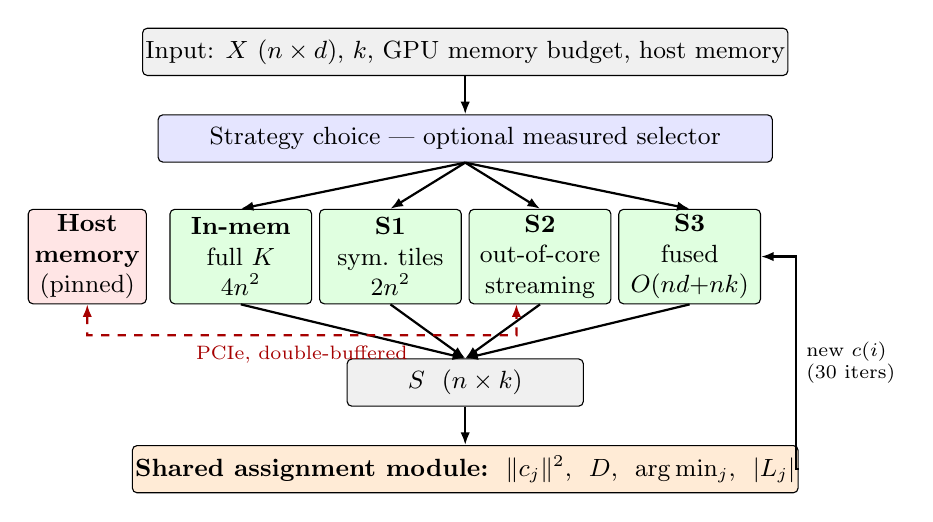
\begin{tikzpicture}[
    x=1mm, y=1mm, font=\small,
    box/.style   = {draw, rounded corners=0.6mm, align=center, inner sep=1pt},
    wide/.style  = {box, minimum width=78mm, minimum height=6mm},
    strat/.style = {box, minimum width=18mm, minimum height=12mm,
                    fill=green!12},
    ar/.style    = {-{Latex[length=1.6mm]}, thick},
  ]

  % ---------- input / selector ----------
  \node[wide, fill=black!6] (in)  at (0,  0)
       {Input: $X$ ($n\times d$), $k$, GPU memory budget, host memory};
  \node[wide, fill=blue!10] (sel) at (0,-11)
       {Strategy choice --- optional measured selector};

  % ---------- the four strategies ----------
  \node[strat] (sA) at (-28.5,-26) {\textbf{In-mem}\\full $K$\\$4n^2$};
  \node[strat] (sB) at ( -9.5,-26) {\textbf{S1}\\sym.\ tiles\\$2n^2$};
  \node[strat] (sC) at (  9.5,-26) {\textbf{S2}\\out-of-core\\streaming};
  \node[strat] (sD) at ( 28.5,-26) {\textbf{S3}\\fused\\$O(nd{+}nk)$};

  % ---------- host memory, beside the strategy row ----------
  \node[box, fill=red!10, minimum width=15mm, minimum height=12mm]
       (hm) at (-48,-26) {\textbf{Host}\\\textbf{memory}\\(pinned)};

  % ---------- S and the shared assignment module ----------
  \node[box, fill=black!6, minimum width=30mm, minimum height=6mm]
       (S) at (0,-42) {$S$\ \ ($n\times k$)};
  \node[wide, fill=orange!16] (asg) at (0,-53)
       {\textbf{Shared assignment module:}\ \
        $\lVert c_j\rVert^2$,\ \ $D$,\ \ $\arg\min_j$,\ \ $\lvert L_j\rvert$};

  % ---------- flow ----------
  \draw[ar] (in) -- (sel);
  \foreach \s in {sA,sB,sC,sD} \draw[ar] (sel.south) -- (\s.north);
  \foreach \s in {sA,sB,sC,sD} \draw[ar] (\s.south) -- (S.north);
  \draw[ar] (S) -- (asg);

  % ---------- host <-> S2 over PCIe ----------
  \draw[{Latex[length=1.6mm]}-{Latex[length=1.6mm]}, thick, dashed, red!65!black]
       (hm.south) -- (-48,-36)
       -- node[midway, below, font=\scriptsize, text=red!65!black]
          {PCIe, double-buffered} (6.5,-36) -- ([xshift=-3mm]sC.south);

  % ---------- iteration loop ----------
  \draw[ar] (asg.east) -- (42,-53) -- (42,-26)
       node[midway, right, font=\scriptsize, align=left]
       {new $c(i)$\\(30 iters)} -- (sD.east);

\end{tikzpicture}}

  \Description{Block diagram: the input and memory budget feed an optional
    selector, which chooses one of four strategies for computing the matrix S;
    all four feed a shared assignment module that loops back with new cluster
    labels.}
  \caption{System block diagram. The optional selector picks one strategy for
    computing $S$; all strategies feed the same assignment module, which loops
    back to the active strategy with new labels each iteration.}
  \label{fig:arch}
\end{figure}

\textbf{Selector.} Takes $n$, $d$, $k$, the GPU memory budget and the available
host memory, and will use measured strategy costs and memory requirements to
choose a strategy before clustering starts. The simple model in
Section~\ref{sec:expected} is an initial hypothesis; a measured selector is a
stretch goal.

\textbf{In-memory path.} Keeps the full $K$ on the device, as Popcorn does, and
is a reference path when it fits the budget. Our own reimplementation provides
a common framework for comparison, although differences in scheduling and
tuning can also affect performance.

\textbf{S1: symmetric tiles.} Stores only the upper-triangular tiles of $K$ on
the GPU, about $2n^2$ bytes. A single pass over a tile produces the
contributions for both $(i,l)$ and $(l,i)$, so no arithmetic is wasted, but the
two contributions land in different rows of $S$. The resulting write conflicts
will be handled either with per-block partial buffers followed by a reduction
or with atomics. We will measure their storage and contention costs, including
diagonal tiles, where each element must be counted once.

\textbf{S2: out-of-core streaming.} Holds the upper-triangular tiles in pinned
host memory and streams them to the GPU every iteration, using several CUDA
streams with double buffering so that PCIe transfers overlap with the
accumulation into $S$. CUDA events will prevent a buffer from being reused
until its copy and compute complete. Contributions from concurrent tiles
require atomics or a separate reduction. The device needs tile buffers in
addition to $X$, $S$, labels, and workspace.

\textbf{S3: on-the-fly fused recomputation.} Never stores $K$ at all. Each
thread block owns a row tile of $X$, loops over column tiles, computes the
$X X^{\mathsf{T}}$ tile in shared memory, applies the kernel function in place,
and accumulates directly into the $S$ columns by cluster in shared memory,
which avoids global atomics on the inner loop. Each block owns its output rows;
a row-tile by $k$ accumulator must fit shared memory, so large $k$ may require
smaller row tiles or multiple passes. The intended footprint is $O(nd + nk)$
plus workspace, independent of $n^2$.

\textbf{Shared assignment module.} Implements
Equations~\eqref{eq:norm}--\eqref{eq:assign}: the centroid norms, the matrix
$D$, the row-wise $\arg\min$, and the new cluster sizes. It then loops back to
the $S$ computation for the next iteration. We fix 30 iterations, as the
Popcorn evaluation does, so that timings compare like with like.

\textbf{OpenMP CPU implementation.} Serves both as the correctness reference
for the GPU strategies and as the CPU baseline for speedup numbers.

Finally, the implementation enforces a \emph{configurable} GPU memory budget
rather than querying free memory. Our development machine is shared, so free
memory changes minute to minute; a fixed budget is what makes the experiments
reproducible and lets us emulate a $24$\,GiB consumer GPU on a $48$\,GiB card.

%% ==========================================================================
\section{Language Selection}

All GPU kernels are written in \textbf{CUDA C++}. The project is specifically
about GPU memory capacity and bandwidth, so we need direct control over exactly
the mechanisms a higher-level model hides: shared memory as an explicit staging
area for tiles, multiple streams and events for copy/compute overlap, pinned
host allocations for full PCIe bandwidth, and launch configuration to trade
occupancy against per-thread state. A directive-based model would let us
express the arithmetic but not the data placement this project is about.

The CPU reference implementation and the CPU baseline use \textbf{OpenMP}
(C++), where shared-memory loop parallelism over the host cores is sufficient
and the code should stay simple enough to be trustworthy.

%% ==========================================================================
\section{Related Work}

Popcorn~\cite{popcorn2025} is our direct point of departure. It makes each
iteration fast through a sparse-linear-algebra reformulation, but keeps $K$
resident and re-reads it every iteration, so it is bounded by GPU memory. We
adopt the mathematical reformulation and target the memory bound it leaves in
place; our in-memory path is essentially its design and serves as our baseline.

Baydoun et al.~\cite{baydoun2018} give CPU and GPU parallel Kernel K-means
implementations. Their code is not publicly available and, as discussed in the
Popcorn paper, their dense formulation scales poorly beyond $k = 2$. Our
strategies are designed around arbitrary $k$ and are evaluated up to $k = 100$.

\textbf{Distributed Kernel K-means.} Bellavita et al.~\cite{bellavita2026}
scale exact Kernel K-means across multiple GPUs in their Vivaldi system, and
compare against a single-GPU sliding-window baseline that recomputes kernel
blocks instead of storing them. We focus on
single-GPU storage, transfer, and fused accumulation trade-offs; where
feasible, we will compare with that baseline and distinguish its blockwise
design from ours.

\textbf{GPU classical K-means.} Kruli\v{s} and
Kratochv\'{\i}l~\cite{krulis2020} analyse and optimise CUDA K-means in detail.
Because classical K-means never forms a kernel matrix, its cost is entirely
different --- $O(nkd)$ per iteration, linear in $n$ --- so their optimisations
address a different bottleneck. Their tuning of the inner loop is nonetheless
a useful reference for ours.

Approximate kernel K-means~\cite{chitta2011} reduces cost by approximating $K$
from a sampled subset of columns. That line of work is orthogonal to ours: it
changes the answer to fit the memory, whereas we keep the exact algorithm and
change how the memory is used.

Dhillon et al.~\cite{dhillon2004} establish Kernel K-means and its relationship
to spectral clustering and normalized cuts, which is why the algorithm is
worth scaling.

The roofline model~\cite{williams2009} underpins our cost model and our
analysis: each strategy is characterised by its arithmetic intensity, and the
crossover dimensions in Section~\ref{sec:expected} compare simplified costs of
different strategies; they are not necessarily roofline ridge points.

Out-of-core processing and the recompute-versus-store trade-off are
long-established HPC techniques; the contribution here is their application to
Kernel K-means and determining when each one wins.

%% ==========================================================================
\section{Statement of Expected Results}
\label{sec:expected}

All development and measurement run on a single NVIDIA RTX A6000
(48\,GiB) on PCIe Gen~4 $\times$16, hosted by a 64-core machine with roughly
1\,TiB of RAM.

\subsection{Predicted problem sizes}

\begin{table}[t]
  \caption{Idealized limits on $n$, fp32, excluding additional allocations.
    S2 is bounded by host memory and S3 by time (60\,s per iteration at
    $d = 50$, $k = 100$), so neither depends on the GPU budget. Capacities use
    $1$\,GiB $= 2^{30}$ bytes.}
  \label{tab:maxn}
  \small
  \begin{tabular}{llrr}
    \toprule
    Strategy & GPU bytes & \multicolumn{2}{c}{max $n$} \\
    \cmidrule(l){3-4}
             & for $K$ & 24\,GiB & 48\,GiB \\
    \midrule
    In-memory (full $K$)  & $4n^2$              & 76{,}145   & 107{,}686 \\
    S1 symmetric tiles    & $2n^2$              & 107{,}686  & 152{,}291 \\
    S2 out-of-core        & host, $2n^2$        & 550{,}268  & 550{,}268 \\
    S3 fused recompute    & $4(nd{+}nk)$        & 3{,}407{,}662 & 3{,}407{,}662 \\
    \bottomrule
  \end{tabular}
\end{table}

With a $10\%$ headroom policy, $M_{\mathrm{gpu}} = 0.9 \times
M_{\mathrm{budget}}$, and a host budget of $80\%$ of available RAM
($M_{\mathrm{host}} = 564$\,GiB at measurement time), idealized limits on $n$
per strategy are given in Table~\ref{tab:maxn}.

Under the simplified formulas, S1 increases the matrix-only limit by
approximately $\sqrt{2}$, and S2 increases it by $3.6\times$ over S1 at
48\,GiB. These are not guaranteed allocation limits: labels, $D$, buffers,
padding and workspace also consume memory. The S2 estimate additionally assumes
that 564\,GiB can be pinned; this must be tested on the shared host. S3 still
has a finite memory limit, though its principal arrays grow linearly in $n$.

\subsection{Cost model}

Counting bytes moved and FLOPs performed per iteration gives
\begin{align}
  T_{\text{in-mem}} &\approx \frac{4n^2}{B_{\mathrm{gpu}}}, &
  T_{\mathrm{S2}}   &\approx \frac{2n^2}{B_{\mathrm{pcie}}}, &
  T_{\mathrm{S3}}   &\approx \frac{2n^2 d}{F_{\mathrm{eff}}}.
  \label{eq:cost}
\end{align}
We have already measured the two bandwidths on the target machine with our own
microbenchmarks: $B_{\mathrm{pcie}} = 26.25$\,GB/s (median of five 1\,GiB
pinned host-to-device copies) and $B_{\mathrm{gpu}} = 679.35$\,GB/s (median of
five runs of a read\,+\,write copy kernel over 1\,GiB). The FP32 peak derived
from the device properties is $38.71$\,TFLOP/s. The fused kernel is not yet
implemented, so we adopt a planning assumption of half of peak,
\begin{equation}
  F_{\mathrm{eff}} = 0.5 \times F_{\text{peak}} = 19.35\ \mathrm{TFLOP/s},
  \label{eq:feff}
\end{equation}
This optimistic assumption must be replaced by measurements. The model also
omits kernel-function evaluation, label-based accumulation, synchronization,
input traffic, assignment, and one-time construction costs; the measured copy
bandwidth is not necessarily the bandwidth of our accumulation kernels. Thus
these figures are illustrative hypotheses, not measured results.

Equating the terms of Equation~\eqref{eq:cost} yields two crossover dimensions.
Recomputation beats streaming when
\begin{equation}
  d < \frac{F_{\mathrm{eff}}}{B_{\mathrm{pcie}}} = 737,
  \label{eq:cross1}
\end{equation}
and recomputation beats re-reading a resident $K$ when
\begin{equation}
  d < \frac{2 F_{\mathrm{eff}}}{B_{\mathrm{gpu}}} = 57.0 .
  \label{eq:cross2}
\end{equation}
Under these assumptions, Equation~\eqref{eq:cross1} suggests recomputation may
outperform streaming for some low-dimensional datasets. Ledgar and SCOTUS in
Popcorn have much larger dimensions; actual crossovers must be measured.
Equation~\eqref{eq:cross2} is the more interesting prediction: at
$d \lesssim 57$, recomputing $K$ from scratch every iteration is predicted by
this simplified model to be faster than reading a stored $K$. Acoustic
($d = 50$) and Letter ($d = 26$, as reported by Popcorn) fall below this
threshold; MNIST ($d = 780$) and CIFAR-10 ($d = 3072$) sit far above it.

\subsection{Worked example}

Take $n = 215{,}373$, twice the in-memory maximum at the 48\,GiB budget, with
$d = 50$. The full $K$ would need $172.8$\,GiB and its upper triangle
$86.4$\,GiB, so neither the in-memory path nor S1 can run this problem. The
model predicts $T_{\mathrm{S2}} = 2n^2 / B_{\mathrm{pcie}} = 3534$\,ms per
iteration against $T_{\mathrm{S3}} = 2n^2 d / F_{\mathrm{eff}} = 240$\,ms, an
illustrative $14.7\times$ ratio before the omitted costs above. The $X$ and $S$
arrays alone occupy $0.12$\,GiB on the device. Over the fixed 30 iterations
that is a predicted $106$\,s versus $7.2$\,s.

For the concrete dataset that motivates the work, Acoustic needs
$4n^2 = 23.15$\,GiB for $K$, so it is predicted \emph{not} to fit the 24\,GiB
budget ($M_{\mathrm{gpu}} = 21.6$\,GiB) and to fit the 48\,GiB budget
($43.2$\,GiB). Under S3 the $X$ and $S$ arrays alone need $0.044$\,GiB at
$k = 100$.

We expect S2 to be transfer-bound in practice: at $d = 50$ the arithmetic that
overlap can hide is small relative to the PCIe time, so double buffering should
recover the compute phase and little else. We therefore report the achieved
overlap fraction alongside the aggregate timing, since that is the quantity
separating a transfer-bound from a latency-bound result.

\subsection{Evaluation plan}

The evaluation measures milliseconds per iteration against $n$, marking the
points where the in-memory path and Popcorn exceed each memory budget; against
$d$, to locate the two crossovers of Equations~\eqref{eq:cross1}
and~\eqref{eq:cross2} and overlay the model predictions; and for
$k \in \{10, 50, 100\}$. Each kernel is placed on a roofline plot, an Nsight
Systems timeline verifies the S2 copy/compute overlap, and if implemented,
selector accuracy is reported as the fraction of configurations for which it
picks the strategy that turns out fastest.

Datasets are synthetic data with controlled $n$, $d$ and $k$, plus the libSVM
sets used by Popcorn (Acoustic, MNIST, Letter, CIFAR-10). We use the polynomial
kernel $(x^{\mathsf{T}} y + 1)^2$, matching Popcorn, fixed initial labels and
deterministic tie-breaking. Empty clusters are excluded from assignment for
that iteration; the same rule is used by every implementation. For small inputs
we compare $S$, centroid norms, distances and objective values with a
higher-precision CPU reference using stated tolerances, including diagonal
tiles, ties, uneven tiles and empty clusters. We compare assignments and
objectives over iterations for $n \le 20{,}000$, investigating near-tie
disagreements caused by floating-point reduction order. Exact means no kernel
approximation, not identical floating-point results or a globally optimal
clustering.

We report construction, iteration and end-to-end time, peak host and device
memory, and CPU speedup versus one thread. GPU profiling will examine
accumulation contention, bandwidth, cluster imbalance, and S2 overlap;
repeated trials and GPU load will be recorded. Comparisons to Popcorn and the
sliding-window baseline include implementation differences. Core deliverables
are a correct shared framework, CPU reference, S2 and S3; S1 and the automatic
selector are stretch goals if time permits.

\subsection{Contributions}

\begin{itemize}
  \item A comparison of out-of-core streaming and fused recomputation for
        exact Kernel K-means, implemented in CUDA; symmetric tiling is a
        stretch goal.
  \item Running problem sizes at which Popcorn exceeds the memory budget on
        the same GPU.
  \item A cost model tested against measurements; an automatic selector if
        time permits.
  \item A re-evaluation of Popcorn's store-and-reread design for
        low-dimensional data, where recomputing is predicted to win.
\end{itemize}

%% ==========================================================================
\section{Timetable}

\begin{table}[H]
  \caption{Project schedule.}
  \label{tab:plan}
  \small
  \begin{tabular}{p{0.26\columnwidth}p{0.62\columnwidth}}
    \toprule
    Period & Work \\
    \midrule
    Oct & Popcorn analysis, target-machine characterisation and bandwidth
          microbenchmarks, baseline reproduction. \\
    Nov, week 1 & Shared framework, data generator, OpenMP CPU reference,
                  in-memory GPU version. \\
    Nov, weeks 2--3 & Correct but unoptimized S2 and S3. \\
    Nov, week 4 & Optimization; S1 and selector if time permits. \\
    Early Dec & Full experiments and cost-model validation; project
                presentation. \\
    Dec 28, 2026 & Final report and source code. \\
    \bottomrule
  \end{tabular}
\end{table}

\paragraph{Division of work.}
賴邑城 (112550009) takes the S3 fused recomputation kernel and the roofline
analysis. 周廷威 (112550013) takes S1 and S2 together with the Nsight timeline
analysis, since both concern data movement. 張程翔 (112550205) takes the shared
framework, the OpenMP CPU version, the Popcorn baseline, the selector and cost
model, and the experiment scripts and plots.

%% ==========================================================================
\bibliographystyle{ACM-Reference-Format}
\bibliography{refs}

\end{document}
